\chapter{超空間與超對稱動力學的構造}

\lectureoverview{我們從超對稱能作用的最小系統出發，重新建構超對稱：一個玻色振子和一個能量相同的費米振子。兩者分別滿足二階和一階方程，這項差異引出超荷及其代數。接著，我們將該代數重新詮釋為座標由普通座標 (t) 和格拉斯曼座標 \(\theta,\bar\theta\) 組成的空間上的幾何。超場將玻色子、費米子和輔助場組合成單一物件；貝列津積分提取出不變的普通拉格朗日量；協變導數使相容於對稱性的約束得以成立；手徵約束則是第一個重要例子。本講刻意呈現這套機制在符號與排序上的難題，最後說明為什麼對稱性本身比費曼規則的彙編更為根本。}

\section{回到單模系統}

讓我們再次從靜止的費米子和玻色子談起。我們省略所有空間座標和動量標記。在給定的模態中，一個量子不是存在就是不存在，只需用創生與湮滅算符便足以描述。以 \(a^\dagger,a\) 表示玻色模態，以 \(c^\dagger,c\) 表示費米模態。它們滿足
\begin{align}
[a,a^\dagger]&=1,
&
\{c,c^\dagger\}&=1,
&
c^2=(c^\dagger)^2&=0.
\end{align}
若兩個量子的能量相同，皆為 \(m\)，那麼除去無關緊要的真空常數後，
\begin{equation}
H=m\left(a^\dagger a+c^\dagger c\right).
\label{eq:l7-one-mode-hamiltonian}
\end{equation}
數目算符 \(a^\dagger a\) 可以取任意非負整數值，而 \(c^\dagger c\) 只能取零或一。這就是這個玩具模型的全部運動學。

這項簡化是策略性的。我們想了解一種操作：在不改變能量的情況下，移除一個玻色子並加入一個費米子，或反過來操作。不過，在建構這種操作之前，我們先把同一個系統從算符語言改寫成拉格朗日量語言。

\section{玻色振子}

對玻色子，引入一個實座標 \(\phi(t)\)。沒有空間變化時，自由標量場就成了一個普通的諧振子。黑板上最初寫下的表示式是
\[
\frac{1}{2}\dot\phi^{,2}+\frac{1}{2}m^2\phi^2.
\]
那是動能加上位能，不是拉格朗日量。講課時立刻修正了符號：
\begin{equation}
L_B=\frac{1}{2}\dot\phi^{,2}-\frac{1}{2}m^2\phi^2.
\label{eq:l7-boson-lagrangian}
\end{equation}

\begin{figure}[H]
\centering
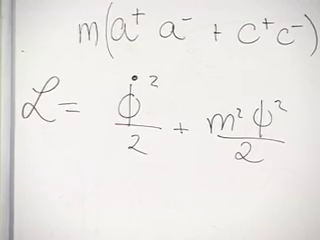
\includegraphics[width=0.62\textwidth]{lecture_07_figure_02.png}
\lectureframe{00:03:25.431}
\caption{位於玻色拉格朗日量上方的單模哈密頓量。畫面保留了口頭修正為 \(T-V\) 之前的初始正號。}
\end{figure}

\begin{classroomqa}
\audiencequestion{所示振子拉格朗日量中的符號有什麼問題？\lecturetimestamp{00:04:00}}
\lecturerresponse{能量是 \(T+V\)，但拉格朗日量是 \(T-V\)。因此，位能項必須帶負號。這項修正使方程從指數變化轉為預期的諧振子振盪。}
\end{classroomqa}

確實，尤拉--拉格朗日方程給出
\begin{align}
\frac{d}{dt}\frac{\partial L_B}{\partial\dot\phi}
&=\frac{\partial L_B}{\partial\phi},\\
\ddot\phi&=-m^2\phi,
\end{align}
也就是
\begin{equation}
\ddot\phi+m^2\phi=0.
\label{eq:l7-boson-eom}
\end{equation}
其頻率是 \(m\)，而不是 \(m^2\)。將這個振子量子化，便會得到與式~\eqref{eq:l7-one-mode-hamiltonian}中由 \(a^\dagger\) 和 \(a\) 描述的相同階梯態。

\section{為什麼費米子作用量是一階的}

費米子拉格朗日量看起來較簡單，因為它只含一個時間導數。從一個刻意簡化的嘗試，已可看出原因。對普通的可交換變數，
\begin{equation}
L_{\mathrm{trial}}=\phi\dot\phi
=\frac{1}{2}\frac{d}{dt}\phi^2.
\end{equation}
這是一個全導數。其尤拉--拉格朗日方程只給出 \(\dot\phi=\dot\phi\)，因此任何可微路徑都符合條件。從作用量中去掉全導數會改變端點資料，但不會改變體內的運動方程。

現在將變數改記為 \(\psi\)，並令它是格拉斯曼奇變數。\(\psi\) 和 \(\dot\psi\) 都會反交換。採用左變分的固定約定時，重新排列奇變數因子會引入負號，因此相同的形式推導得到
\begin{equation}
\frac{d}{dt}\frac{\partial L_{\mathrm{trial}}}{\partial\dot\psi}
=\dot\psi,
\qquad
\frac{\partial L_{\mathrm{trial}}}{\partial\psi}
=-\dot\psi.
\end{equation}
所以方程為
\begin{equation}
\dot\psi=-\dot\psi
\quad\Longrightarrow\quad
\dot\psi=0.
\label{eq:l7-constant-fermion}
\end{equation}
對可交換座標而言只是同義反覆的表示式，對反交換座標卻有了動力學意義。對振子來說，這個方程施加了過多限制，因為它只允許常數解；但這正是我們需要的線索。

\begin{classroomqa}
\audiencequestion{解真的就只是 \(\psi\) 為常數嗎？\lecturetimestamp{00:13:57}}
\lecturerresponse{是的。式~\eqref{eq:l7-constant-fermion} 是一個真正的一階微分方程，其解是任意的格拉斯曼值常數。加入質量項，就能把這個靜態解變成振盪解。}
\end{classroomqa}

顯而易見的嘗試 \(m\psi^2\) 之所以行不通，是因為 \(\psi^2=0\)。我們需要兩個實奇變數 \(\psi_1,\psi_2\)，或者等價地，使用一個複變數及其共軛。講課時在黑板上逐步推導雙實變數形式，並反覆核對符號和因子二。依照慣例正規化的複數形式為
\begin{equation}
L_F=\frac{i}{2}
\left(\bar\psi\dot\psi-\dot{\bar\psi}\psi\right)
-m\bar\psi\psi.
\label{eq:l7-fermion-lagrangian}
\end{equation}
除去一個全導數後，這就是 \(i\bar\psi\dot\psi-m\bar\psi\psi\)。對 \(\bar\psi\) 作變分，得到
\begin{equation}
i\dot\psi=m\psi,
\qquad
\psi(t)=\psi(0)e^{-imt}.
\label{eq:l7-fermion-eom}
\end{equation}
共軛方程的相位則相反。因此，費米子模態也以能量 \(m\) 振盪，與玻色子模態相同，儘管它的方程是一階而非二階。

\editorialnote{~\eqref{eq:l7-fermion-lagrangian} 為探索性的雙實變數計算採用了一種標準排序與正規化。講課時則加入因子 \(i\)、調整一個因子二，並留下某個實分量的符號未定。這些變動不影響核心結論：費米子動力學是一階的，質量以線性形式出現，而複費米子具有非零的雙線性項。}

這是熟悉的相對論性對比在零維情況下的縮影。Klein--Gordon 方程對時間是二階的，而 Dirac 方程是一階的。省略空間後，玻色子是諧振子，費米子則是複數格拉斯曼振子。

\begin{classroomqa}
\audiencequestion{\(\psi\)、\(\dot\psi\)及其共軛的書寫順序重要嗎？\lecturetimestamp{00:18:58}}
\lecturerresponse{中間推導確實會受排序影響，因為奇變數因子會反交換。只要全程採用一致的左變分或右變分、共軛和積分約定，物理理論就不會依賴任意的書寫偏好。交換一對奇變數因子會改變符號，而其他地方也必須一致地調整。}
\end{classroomqa}

結合式~\eqref{eq:l7-boson-lagrangian}和\eqref{eq:l7-fermion-lagrangian}，便能以拉格朗日量描述式~\eqref{eq:l7-one-mode-hamiltonian}所代表的同一組等能配對。現在可以找出它們之間的對稱性了。

\section{超荷及其代數}

移除費米子並加入玻色子的算符為
\begin{equation}
Q^\dagger=\sqrt{2m}\,a^\dagger c,
\end{equation}
其共軛算符則移除玻色子並加入費米子：
\begin{equation}
Q=\sqrt{2m}\,a c^\dagger.
\end{equation}
我們選擇此正規化，使代數具有標準形式。利用 \(cc^\dagger=1-c^\dagger c\)、\(aa^\dagger=a^\dagger a+1\)，以及玻色算符與費米算符彼此可交換這項性質，
\begin{align}
\{Q,Q^\dagger\}
&=2m\left(ac^\dagger a^\dagger c+a^\dagger c a c^\dagger\right)\notag\\
&=2m\left[(a^\dagger a+1)c^\dagger c
+a^\dagger a(1-c^\dagger c)\right]\notag\\
&=2m\left(a^\dagger a+c^\dagger c\right)=2H.
\label{eq:l7-superalgebra}
\end{align}
玻色算符可以移過費米算符。同樣的冪零性限制了費米子的佔據數，並給出
\begin{equation}
Q^2=(Q^\dagger)^2=0.
\end{equation}
最後，
\begin{equation}
[H,Q]=[H,Q^\dagger]=0.
\label{eq:l7-conserved-supercharges}
\end{equation}
每個超荷都以相反方向改變玻色子數和費米子數，因此頻率相同時，兩者造成的能量變化會相消。

\begin{classroomqa}
\audiencequestion{\([H,Q]\) 是什麼？答案會與 \(Q\) 成正比嗎？\lecturetimestamp{00:25:10}}
\lecturerresponse{不，答案是零。單獨的創生或湮滅算符與 \(H\) 對易時，會帶出其能量；但在 \(Q\) 中，玻色子和費米子的貢獻彼此相消。這項相消正是兩者能量相同的結果。}
\end{classroomqa}

\begin{classroomqa}
\audiencequestion{那個對易子不是已經寫在黑板上了嗎？\lecturetimestamp{00:25:45}}
\lecturerresponse{是的。重新推導一次很有用，因為這迫使我們理解這個關係，而不只是照抄：與哈密頓量對易表示該變換是對稱變換，其生成元守恆。}
\end{classroomqa}

「\emph{荷}」一詞反映了這項守恆律。不過，我們不應把 \(Q\) 視為附著在態上的普通數值，也不能把它當成可與其他量同時測量的數值。它是格拉斯曼奇、冪零的算符，會將玻色態映射成費米態。較準確的說法是：它是作用於簡併超多重態中的守恆生成元。
\editorialnote{這樣的措辭修正了課堂上以能量或電荷為態標記的類比。單個非厄米奇超荷不是具有數值量子標記的普通可觀測量。正確的分類依據是它們的守恆作用，以及整個超代數的表示。}

\section{作為導數的生成元}

這個代數很簡潔，但單靠它本身，還無法告訴我們如何建構交互作用理論。下一步是從幾何著手。熟悉的對稱性生成元本來就以微分算符的形式作用。按照講課採用的約定，
\begin{equation}
H=i\frac{\partial}{\partial t},
\qquad
P=-i\frac{\partial}{\partial x}.
\end{equation}

\begin{figure}[H]
\centering
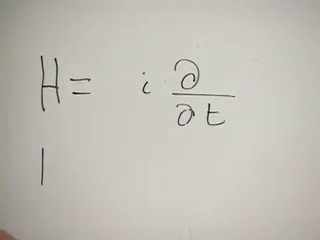
\includegraphics[width=0.50\textwidth]{lecture_07_figure_03.png}
\lectureframe{00:28:12.720}
\caption{哈密頓量表示為時間平移的生成元。}
\end{figure}

角動量同樣是座標與導數的乘積。若超荷是奇生成元，自然會想知道能否用對奇座標微分的方式表示。因此，我們將時間軸擴展為超空間
\begin{equation}
(t,\theta,\bar\theta),
\qquad
\theta^2=\bar\theta^2=0,
\qquad
\theta\bar\theta=-\bar\theta\theta.
\end{equation}
定義在這個空間上的場，依賴普通時間及一對互為共軛的格拉斯曼座標。

本講刻意呈現符號有多容易出錯。複共軛引入的符號、移動奇參數引入的符號，以及選擇左導數而非右導數引入的符號，是三種不同的操作。為避免保留彼此不相容的黑板推導階段，我們現在固定一種約定：所有奇導數都是左導數，並且
\begin{equation}
q=\partial_\theta+i\bar\theta\partial_t,
\qquad
\bar q=\partial_{\bar\theta}+i\theta\partial_t.
\label{eq:l7-differential-supercharges}
\end{equation}
於是
\begin{equation}
q^2=\bar q^{,2}=0,
\qquad
\{q,\bar q\}=2i\partial_t=2H.
\label{eq:l7-differential-algebra}
\end{equation}
因子二來自兩個交叉項：\(\{\partial_\theta,\theta\}=1\)和\(\{\partial_{\bar\theta},\bar\theta\}=1\)。若生成元只含 \(\partial_\theta\) 和 \(\partial_{\bar\theta}\)，它們的反對易子就會是零，無法重現哈密頓量。

\begin{classroomqa}
\audiencequestion{\(q\)和\(\bar q\)中的兩個時間導數項應該帶相同的符號嗎？\lecturetimestamp{00:31:01}}
\lecturerresponse{必須一致選定兩項的符號，才能使混合反對易子等於 \(2H\)。可以採用整體正號的約定，也可以採用與之共軛且始終一致的另一種約定。相對符號應由計算決定，不能憑對符號 \(i\) 的視覺直覺判斷。}
\end{classroomqa}

教室裡一再核對符號，這種困難後來成了笑話：符號好像在通勤上班途中就變了。這個笑話很貼切。讓格拉斯曼參數穿過座標時，反交換可能改變符號，即使物理約定並沒有改變。式~\eqref{eq:l7-differential-supercharges}是後續內容一律採用的固定依據。

\subsection{超對稱性作為座標平移}

令 \(\xi,\bar\xi\) 為無窮小奇參數。按照上述約定，以
\begin{equation}
\delta_\xi=\xi q+\bar\xi\bar q
\end{equation}
作用於超場，等價於施行下列無窮小座標變換：
\begin{align}
\theta&\longrightarrow\theta+\xi,\\
\bar\theta&\longrightarrow\bar\theta+\bar\xi,\\
t&\longrightarrow t+i\left(\xi\bar\theta+\bar\xi\theta\right).
\label{eq:l7-coordinate-shift}
\end{align}
因此，標量超場的變化為
\begin{equation}
\delta_\xi\Phi
=\left(\xi\partial_\theta+\bar\xi\partial_{\bar\theta}
+i\xi\bar\theta\partial_t+i\bar\xi\theta\partial_t\right)\Phi
=\left(\xi q+\bar\xi\bar q\right)\Phi.
\end{equation}
這就是超對稱性的幾何內涵：奇方向上的平移與普通時間平移相連。由於式~\eqref{eq:l7-differential-algebra}，兩個奇平移的合成會閉合為時間平移。

\begin{classroomqa}
\audiencequestion{有爭議的負號是否代表時間向後平移？\lecturetimestamp{00:58:13}}
\lecturerresponse{不同的符號約定可以使寫出的無窮小時間平移方向相反，但這並未引入另一種物理上的逆時過程。關鍵在於，座標變換和微分生成元必須遵守同一個代數。}
\end{classroomqa}

\begin{classroomqa}
\audiencequestion{這種延伸的時間有物理實現嗎？還是只是一種形式上的記帳方式？\lecturetimestamp{00:58:23}}
\lecturerresponse{從一個有用的角度來看，它是一種記帳方式：用幾何形式整理代數。但引入交互作用後，這種整理就有了物理價值。超空間提供系統化的演算，讓我們能逐步建構出保持玻色子--費米子對稱性的拉格朗日量，正如張量演算有助於建構洛倫茲純量。}
\end{classroomqa}

\section{超場與輔助分量}

由於只有兩個奇座標，偶超場的展開會終止：
\begin{equation}
\Phi(t,\theta,\bar\theta)
=\phi(t)+\bar\theta\psi(t)+\bar\psi(t)\theta
+D(t)\bar\theta\theta.
\label{eq:l7-superfield}
\end{equation}
偶單項式 \(\phi\) 和 \(D\) 的係數是玻色量；奇單項式 \(\psi\) 和 \(\bar\psi\) 的係數是費米量。\(\theta^2\)、\(\bar\theta^2\)以及更高次項都不會留下。我們不展開時間依賴，因為對 \(t\) 作普通泰勒展開不會終止，而且在此也沒有必要。

\begin{classroomqa}
\audiencequestion{最高項中的分量 \(D(t)\) 是什麼？\lecturetimestamp{00:41:46}}
\lecturerresponse{此時它只是有限展開中最後一個玻色係數。在分量作用量中，它通常沒有動能項，並透過代數運動方程消去，因此稱為輔助場。本講開玩笑地建議用 ``D 表示 dummy（虛設量），''這點出了它不具動力學的角色，但不是此名稱的歷史由來。}
\end{classroomqa}

超場是單一物件，而 \(\phi,\psi,\bar\psi,D\) 是它的分量。超對稱變換會將這些分量混合。因此，玻色子與費米子的關係，在結構上很像向量的 \(x\) 分量和 \(y\) 分量透過旋轉相互關聯；不過，格拉斯曼方向無法想像成普通的座標軸。

\section{超作用量與最高分量}

要求得運動方程，我們需要作用量。在普通場論中，先構造純量拉格朗日量，再對時空積分。這裡對應的表示式是
\begin{equation}
S=\int dt\,d\theta\,d\bar\theta\;\Lambda
\bigl(\Phi,\text{ superspace derivatives of }\Phi\bigr),
\label{eq:l7-superaction}
\end{equation}
其中 \(\Lambda\) 是偶超場。貝列津積分是代數運算。我們選定
\begin{equation}
\int d\theta\,d\bar\theta\;\bar\theta\theta=1.
\end{equation}
因此，若
\begin{equation}
\Lambda=A+\bar\theta B+\bar B\theta+C\bar\theta\theta,
\end{equation}
則
\begin{equation}
\int d\theta\,d\bar\theta\;\Lambda=C.
\label{eq:l7-top-component}
\end{equation}
對奇座標積分會提取最高分量，留下普通拉格朗日量，再對時間積分。

為什麼結果具有不變性？超對稱變分會平移積分變數。最高分量的變分是時間上的普通全導數，而奇方向的全導數在貝列津積分下為零。在適當的端點條件下，作用量不變。這相當於先建構洛倫茲純量、再對時空積分的超空間版本。

\section{超場的乘積}

從舊超場構造新超場，最簡單的方法就是將它與自身相乘。從式~\eqref{eq:l7-superfield}出發，所有含有 \(\theta^2\) 或 \(\bar\theta^2\) 的項都會消失。維持 \(\bar\theta\theta\) 的排序，並將帶橫線的分量場置於左側，得到
\begin{align}
\Phi^2
={}&\phi^2
+2\phi\bar\theta\psi
+2\phi\bar\psi\theta\notag\\
&+\left(2\phi D-2\bar\psi\psi\right)\bar\theta\theta.
\label{eq:l7-superfield-square}
\end{align}

\begin{figure}[H]
\centering
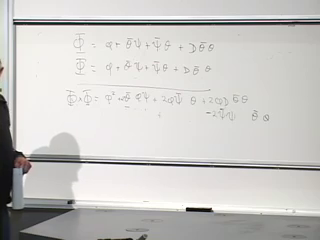
\includegraphics[width=0.82\textwidth]{lecture_07_figure_05.png}
\lectureframe{01:07:57.844}
\caption{逐分量展開的超場乘積，以及其中的 \(\bar\theta\theta\) 項。}
\end{figure}

兩項 \(\phi D\) 和 \(D\phi\) 會相加，因為兩個場都是偶的。兩個費米子交叉項在各自重新排序後也會相加，但共同的符號是負號：
\begin{equation}
(\bar\theta\psi)(\bar\psi\theta)
+(\bar\psi\theta)(\bar\theta\psi)
=-2\bar\psi\psi\,\bar\theta\theta.
\end{equation}
對平方項作奇座標積分，得到
\begin{equation}
\int d\theta\,d\bar\theta\;\Phi^2
=2\phi D-2\bar\psi\psi.
\end{equation}
這一項依照建構方式具有超對稱性，但還不是動能拉格朗日量，因為它不含時間導數。

接著，講者在黑板上提出 \(\Phi^3\)、\(\Phi^4\) 和 \(\Phi^n\) 作為練習，並給出一條簡潔規則。對任意普通函數 \(W\)，
\begin{equation}
\left.W(\Phi)\right|_{\bar\theta\theta}
=W'(\phi)D-W''(\phi)\bar\psi\psi.
\label{eq:l7-function-top-component}
\end{equation}
當 \(W(\phi)=\phi^2\) 時，這會重現式~\eqref{eq:l7-superfield-square}；當 \(W(\phi)=\phi^n\) 時，則得到
\begin{equation}
\left.\Phi^n\right|_{\bar\theta\theta}
=n\phi^{n-1}D-n(n-1)\phi^{n-2}\bar\psi\psi.
\end{equation}
\editorialnote{講者將 \(n\) 次方留作練習，並指出預期會出現哪些類型的項。式~\eqref{eq:l7-function-top-component}則依照固定的排序約定，給出完整規則。}

這時講者問聽眾是否累了。聽眾回答沒有，他則說自己累了。這段對話不只是插科打諢。超場的冪次很容易處理，因為展開會終止；真正棘手的是導數和約束中的符號整理。

\section{哪些導數尊重超對稱性？}

接著討論黑板上的推導之前，先更正一點。普通時間導數沒有問題：
\begin{equation}
[\partial_t,q]=[\partial_t,\bar q]=0.
\end{equation}
因此，只要 \(\Phi\) 是超場，\(\partial_t\Phi\) 也會依照超場的方式變換。較微妙的是裸奇導數 \(\partial_\theta\Phi\) 和 \(\partial_{\bar\theta}\Phi\)，因為它們不會與兩個超荷都反對易。要施加約束並明確地建構超對稱分量，我們需要改造奇導數。
\editorialnote{在此採用的約定下，口頭聲稱時間微分無法產生另一個超場並不正確。由於 \(\partial_t\) 與兩個超荷都對易，它是協變的。後續建構改造後的奇導數仍有必要，這才是本講真正的數學要點。}

\subsection{「``魔法場''」的類比}

講者以普通旋轉說明這項判準。令 \(f(x,y)\) 滿足
\begin{equation}
\partial_y f=0.
\label{eq:l7-magic-constraint}
\end{equation}
稱這類函數為``「魔法場」。''它依賴 \(x\)，但不依賴 \(y\)。魔法場這一類函數在旋轉下是否仍保持？對於
\begin{equation}
L_z=-i\left(x\partial_y-y\partial_x\right),
\end{equation}
我們得到
\begin{equation}
[\partial_y,L_z]=i\partial_x\neq0.
\end{equation}
因此，即使 \(f\) 起初滿足式~\eqref{eq:l7-magic-constraint}，\(L_z f\) 通常仍會產生 \(y\) 依賴性。這項約束並非旋轉不變。

一般原則很簡單。若一個場滿足 \(C\Phi=0\)，而對稱性由 \(G\) 生成，那麼只要 \(C\) 與 \(G\) 的分次對易子為零，變換後的場仍會滿足約束。對兩個奇算符而言，分次對易子就是反對易子。

\begin{classroomqa}
\audiencequestion{場上的約束何時與對稱性相容？\lecturetimestamp{01:17:56}}
\lecturerresponse{當約束算符與對稱性生成元分次對易時。如此一來，\(C(G\Phi)\) 可以將 \(G\) 移到另一側，並化為 \(G(C\Phi)=0\)。旋轉的例子之所以不成立，是因為 \(\partial_y\) 不與旋轉生成元對易。}
\end{classroomqa}

\subsection{協變奇導數}

依照式~\eqref{eq:l7-differential-supercharges}固定超荷後，定義
\begin{equation}
\mathcal D=\partial_\theta-i\bar\theta\partial_t,
\qquad
\bar{\mathcal D}=\partial_{\bar\theta}-i\theta\partial_t.
\label{eq:l7-covariant-derivatives}
\end{equation}
唯一的差異是時間導數項的符號。直接計算得到
\begin{align}
\{\mathcal D,q\}
&=\{\mathcal D,\bar q\}
=\{\bar{\mathcal D},q\}
=\{\bar{\mathcal D},\bar q\}=0,\\
\{\mathcal D,\bar{\mathcal D}\}&=-2i\partial_t.
\label{eq:l7-covariant-algebra}
\end{align}
兩個可能不為零的交叉項會互相抵消。這是奇方向上的協變導數：它在執行微分的同時，保留場的變換規律。

講課時，\(D\)同時用來表示輔助分量和這個導數。我們以\(D(t)\)表示分量，以花體的\(\mathcal D\)表示算符。

\section{手徵約束}

現在可以施加一個在超對稱變換下仍能成立的非平凡約束：
\begin{equation}
\bar{\mathcal D}\Phi=0.
\label{eq:l7-chiral-constraint}
\end{equation}
滿足此條件的場稱為手徵場。若某個場在超對稱變換前是手徵場，則
\begin{equation}
\bar{\mathcal D}(q\Phi)
=-q(\bar{\mathcal D}\Phi)=0,
\qquad
\bar{\mathcal D}(\bar q\Phi)
=-\bar q(\bar{\mathcal D}\Phi)=0.
\end{equation}
因此，變換後的整個超場仍屬於受約束的場類。手徵條件不像魔法場條件，能與此對稱性相容。

為求解此約束，定義平移後的時間座標
\begin{equation}
\tau=t+i\bar\theta\theta.
\label{eq:l7-chiral-time}
\end{equation}
由於我們使用左導數，
\begin{equation}
\partial_{\bar\theta}\tau=i\theta,
\end{equation}
因此
\begin{equation}
\bar{\mathcal D}F(\tau,\theta)
=\left(\partial_{\bar\theta}-i\theta\partial_t\right)F(\tau,\theta)
=i\theta\partial_\tau F-i\theta\partial_\tau F=0.
\end{equation}
一般的局域手徵超場只透過 \(\tau\) 依賴 \(\bar\theta\)：
\begin{equation}
\Phi_{\mathrm{ch}}(\tau,\theta)
=\phi(\tau)+\bar\psi(\tau)\theta.
\label{eq:l7-chiral-field-tau}
\end{equation}

\begin{classroomqa}
\audiencequestion{只有依賴 \(\tau\) 和 \(\theta\) 這種形式，才能滿足手徵約束嗎？\lecturetimestamp{01:32:35}}
\lecturerresponse{局域而言，是的。微分方程 \(\bar{\mathcal D}\Phi=0\) 正表示獨立的 \(\bar\theta\) 依賴可吸收到平移後的座標 \(\tau=t+i\bar\theta\theta\) 中。剩下的有限展開是 \(\tau\) 的函數，再加上一個與 \(\theta\) 成正比的項。}
\end{classroomqa}

改用原來的時間座標重新展開，
\begin{align}
\phi(\tau)
&=\phi(t)+i\bar\theta\theta\dot\phi(t),\\
\bar\psi(\tau)\theta
&=\bar\psi(t)\theta,
\end{align}
因為第二行的修正項含有 \(\theta^2\)。因此，
\begin{equation}
\Phi_{\mathrm{ch}}(t,\theta,\bar\theta)
=\phi(t)+\bar\psi(t)\theta
+i\bar\theta\theta\dot\phi(t).
\label{eq:l7-chiral-field-components}
\end{equation}

\begin{classroomqa}
\audiencequestion{\(\phi(t+i\bar\theta\theta)\)的泰勒展開應該包含二階項嗎？\lecturetimestamp{01:33:51}}
\lecturerresponse{不需要。第一個修正項是 \(i\bar\theta\theta\dot\phi\)，而所有更高階修正項都含有 \((\bar\theta\theta)^2=0\)。聽眾立刻指出這點：冪零性已產生前兩項，並使級數就此終止。}
\end{classroomqa}

這就是手徵性的精簡之處。式~\eqref{eq:l7-superfield}中的未受約束超場有兩個玻色分量槽和兩個費米分量槽。在這個最小的一維例子中，手徵條件移除了獨立的輔助分量槽，並將最高分量與\(\dot\phi\)連結起來。

\section{適時停止的計算}

自然的下一步是將手徵場與其共軛相乘，再對超空間積分。講者開始寫共軛場的展開式時，一位聽眾問，共軛後 \(\theta\bar\theta\) 的順序是否必須反轉。此時符號已經不太可靠。講者沒有勉強作答，而是停下計算。

\begin{classroomqa}
\audiencequestion{即使延後共軛場的乘法，能否先說明關鍵結論？\lecturetimestamp{01:37:30}}
\lecturerresponse{可以。只要一致處理符號與共軛，由手徵場及其共軛構成的超空間表示式，就會產生所需的普通玻色與費米動能項。本講的重要成果是建構原理，而不是從疲憊推導中照抄不可靠的最後一行。}
\end{classroomqa}

應該保留這個停止點。這套形式體系不容出錯：一個奇因子的位置不對，就會改變符號；而共軛、微分、乘法和積分必須始終遵守同一套約定。若無法確保整個推導鏈條一致，正確做法是先修正，再繼續。在標準約定下，熟知的動能作用量由共軛乘積建構而成；但詳細的分量化簡應留待下一次完整推導，不宜從未完成的黑板式子中重建。

\section{為什麼對稱性才是重點}

超對稱拉格朗日量不只是把玻色子和費米子並列而已。它會約束兩者的質量與交互作用，使它們構成超代數的一個表示。在精確超對稱的真空中，同一超多重態的成員具有相同質量。它們的圈圖貢獻彼此關聯，而玻色子與費米子的紫外效應會依照對稱性所要求的精確組合相消。

這就是建構方法重要的原因。我們可以列出費曼頂點，再逐個圖形驗證相消，但如此一來，相消便像是偶然發生。超對稱性說明了這些相消的原因，正如洛倫茲對稱性說明散射振幅為何在所有慣性座標系中都遵循一致的變換規律。

\editorialnote{精確超對稱並不表示每一項個別的自能修正都會消失。它會關聯各種重整化，並消除特定的紫外敏感性；不重整化定理的適用範圍則取決於所討論的物理量、時空維度和超對稱數量。本講關於廣泛相消的說法，應保留這些限定。}

\begin{classroomqa}
\audiencequestion{``chiral''怎麼拼？\lecturetimestamp{01:39:48}}
\lecturerresponse{C-H-I-R-A-L。這個詞描述約束\(\bar{\mathcal D}\Phi=0\)，不是指三維空間物體一般所說的幾何手性；不過，此術語的源頭確實與相對論性旋量的左手和右手結構有關。}
\end{classroomqa}

\begin{classroomqa}
\audiencequestion{能不能跳過拉格朗日量，直接使用超對稱費曼規則？\lecturetimestamp{01:40:00}}
\lecturerresponse{當然可以直接列出規則，但如此一來，耦合之間的關係及其所導致的相消，就會像是無法解釋的巧合。更深層的內涵是廣義的時空對稱性。拉格朗日量或等價的不變形式，能揭示其中原因並有系統地導出這些規則。}
\end{classroomqa}

假設每一個微擾階都碰巧給出洛侖茲不變的振幅，儘管從未提及洛侖茲變換。經過足夠多的計算後，我們會要求一個解釋。答案會是能同時組織所有階的時空對稱性。超空間的作用也類似：\(\theta,\bar\theta\)中的位移會混合玻色與費米分量，而其代數會閉合於時空平移。

\begin{classroomqa}
\audiencequestion{普通空間座標是否也應像格拉斯曼座標一樣，展開成有限冪級數？\lecturetimestamp{01:44:55}}
\lecturerresponse{不會。普通座標的冪級數不會終止，通常也不是自然的分解方式。傅立葉變換更有用，因為它能將場分解成波與動量。對\(\theta\)展開之所以特殊，正是因為冪零性使展開在有限項後終止。}
\end{classroomqa}

\begin{classroomqa}
\audiencequestion{如果大型強子對撞機（LHC）出現一種新粒子，我們要如何判斷它是超伴粒子，而不只是某種未知粒子？\lecturetimestamp{01:45:42}}
\lecturerresponse{超對稱預言的是彼此關聯的量子數與相互作用，而不只是一個額外的粒子態。自旋相差二分之一，規範荷彼此關聯；許多三次與四次耦合所需的獨立參數，也比一般理論少。截面、分支比以及其餘粒子譜都必須符合這些關係。}
\end{classroomqa}

單一個陌生的共振態本身不足以證明超對稱；一整套耦合關係與粒子譜關係才足以構成證據。這正是超空間構造在實驗上的對應：表面上彼此獨立的分量相互作用，都源自同一個不變物件。

\begin{classroomqa}
\audiencequestion{觀測到的粒子與其假想的超對稱伴粒子，質量並不相等。這會如何改變理論？\lecturetimestamp{01:47:01}}
\lecturerresponse{改變極大。超對稱必須破缺，而通常是透過自發破缺，再將破缺效應傳遞到可觀測部門。破缺會使多重態中的粒子質量分裂，同時保留足夠的結構來控制相互作用；若破缺尺度夠低，也能控制紫外修正。釐清這套機制本身就是一項龐大的理論工作，尤其是在納入引力時。}
\end{classroomqa}

\section{原理簡單，計算繁難}

結尾的評述格外坦率。起點聽來很簡單：玻色子與費米子由一種對稱性聯繫起來。然而，實際建構很快就成了處理指標、共軛、格拉斯曼變數排列次序與正負號的學問。即使建構出這種對稱性，現實的粒子物理仍需要讓它破缺；將它與引力耦合則會引向超引力，並增添另一層結構。

這種困難並不代表這個想法空洞。大自然沒有義務讓簡單的原理易於計算。專家透過一再處理細節來學習這門學問，直到符號規則變得熟稔自然。令人挫折之處，在於精簡的代數
\begin{equation}
\{Q,Q^\dagger\}=2H
\end{equation}
與在相互作用理論中實現它所需的大量技術細節之間，存在著一段距離。

\begin{classroomqa}
\audiencequestion{再多一層抽象，最終能簡化形式體系嗎？還是複雜性會不斷累積？\lecturetimestamp{01:49:33}}
\lecturerresponse{目前沒有任何一般性的簡化能免除繁複的細節工作。底層規則或許簡短，但要可靠地運用它們，就必須反覆掌握各種約定。這就是為什麼完整講授這門學問，通常得用上一整門技術課程，而不是廣泛涵蓋粒子物理的課程中的一小部分。}
\end{classroomqa}

\begin{classroomqa}
\audiencequestion{這些變換能告訴我們費米子與玻色子究竟是什麼，或是為什麼它們通常呈現不同的行為嗎？\lecturetimestamp{01:51:42}}
\lecturerresponse{它們告訴我們，兩者是同一個超場的分量，並且在超荷作用下互為映像。作用\(Q\)會將玻色分量映射為費米分量；再進行一次變換，則會產生導數與輔助分量。這類似於旋轉混合向量的各個分量，但不能將它轉化成同樣字面的圖像：適當的描述方式是格拉斯曼幾何本身。}
\end{classroomqa}

這個回答讓我們回到核心思想。超對稱變換是超空間中的微小變換。它會混合\(\phi,\psi,\bar\psi,D\)，如同普通旋轉會混合各個分量；而這些變換的代數會閉合為時間平移。這個圖像雖然抽象，卻並非任意構造：超場中的每一項、協變導數中的每個符號，以及分量相互作用之間的每種關係，都是為了實現這套代數而存在。

\section{我們建構了什麼}

我們從相配的振子哈密頓量出發，並找回它的兩種不同拉格朗日描述。玻色子滿足二階振子方程；費米子則需要一階格拉斯曼作用量，以及一對複數的奇分量。超荷會交換這兩個模式，各自平方為零；它們的反對易子給出哈密頓量，且各自與哈密頓量對易。

將這些荷表示為微分算符，便引出了超空間。有限的超場展開將玻色、費米與輔助分量組合起來；別列津積分選出超拉格朗日量的最高分量；乘法則產生可能的不變相互作用項。接著，為了要求奇導數與對稱性相容，我們引入\(\mathcal D,\bar{\mathcal D}\)、手徵約束，以及位移後的座標\(\tau=t+i\bar\theta\theta\)。

尚未完成的共軛乘積計算，也是這一課的一部分，並非需要掩飾的缺陷。超對稱起源於簡單的物理要求，但其微積分對每一種排列次序都很敏感。掌握這些次序後，便能得到豐厚的成果：對稱性組織了質量與耦合，量子修正滿足並非偶然的關係，而玻色子與費米子則成為同一個幾何物件的分量。
